\documentclass[aps,prl,twocolumn,superscriptaddress]{revtex4-1}

% the percent sign gives comments in Latex
% top line indicates this is for Physical Review, standard journal format,
% suitable for electronic submission of articles
%
% the line above is necessary to start any latex document.
% this is one variation that should work for most things.
% if you want double spaceing, use the following:
%
%\documentclass[prd,preprint,letterpaper]{revtex4}
%
% the "preprint" designation will make a wider line
% spacing, good for markup.
\usepackage{amssymb}   % for math
\usepackage{verbatim}  % for the comment environment
\usepackage{color}
\usepackage{float}  	% allows use of 'H' command
\usepackage{flushend}	% makes bibliography balanced
\usepackage{import} 	% to import images as .tex (enriques method)
\usepackage{graphicx}  % this is the up-to-date package for all figures
\usepackage{epstopdf}	% to import images as .tex (enriques method)

%%%
%\usepackage{hyperref}  % needed to add hyperlinks
%\hypersetup{
%  colorlinks=true,
%  linkcolor=blue,
%  filecolor=magenta,
%  urlcolor=cyan,
%}



% LETS YOU DRAW
\usepackage{tikz}




% these are some custom control of the page size and margins
% \topmargin= 0.2in  % these 1st two may be needed for some computers
% \textheight=8.75in
\textwidth=6.5in
%\oddsidemargin=0cm
%\evensidemargin=0cm

% this is where the actual document itself (rather than control statements) begins:

\begin{document}



\title{X-Ray Diffraction}


\author{Corey Mutnik}
\email{cmutnik@hawaii.edu}
\affiliation{Department of Physics \& Astronomy, \\
University of Hawaii at Manoa,\\
2505 Correa Rd, Honolulu, HI, 96822, USA}
\altaffiliation{Quantum Mechanics Lab}




\begin{abstract}
%The experimentally determined lattice constant of NaCl, $a=(599.89\pm35.32)~pm$, deviates from the accepted value of $564.02~pm$ by $1.02\sigma$. % DETERMINED WITHOUT USING NI FILTER K\alpha VALUES IN WEIGHT MEAN

Using X-ray diffraction, crystal structure and lattice constants of NaCl and LiF, were experimentally determined.  The experimentally determined lattice constant of NaCl, $a_{0}=(521.17\pm67.11)~pm$, deviates from the accepted value of $564.02~pm$ by less than $1\sigma$.  The experimentally determined lattice constant of LiF was $a_{0}=(428.44\pm117.10)~pm$.  This deviates from the accepted value of $402.6~pm$ by less than $1\sigma$. 




\end{abstract}

\maketitle    



\section{Introduction}

%%%Bragg’s law of reflection describes the diffraction of plane
%%%waves at a monocrystal as the selective reflection of the waves
%%%at a set of lattice planes within the crystal.

Using Bragg diffraction, the $K_{\alpha}$ and $K_{\beta}$ peaks of two cubic crystals were analyzed.  This was done to determine both crystal structure and respective lattice constant, $a_{0}$, of NaCl and LiF.  Such regular crystalline structures are classified by their unit cells - the smallest volumetric structure containing the necessary information for constructing the entire solid.  Identifying the unit cell required using the Bragg condition:
\begin{center}
	$n\lambda = 2d sin\theta$
\end{center}
where $n$ is the order, $\lambda$ is the wavelength, $d$ is the lattice spacing, 
and $\theta$ is the diffraction angle.  Maximums and minimums in the diffraction pattern give insight into the atomic structure.  For cubic crystals, the lattice constant, $a_{0}$, is twice the lattice spacing:
\begin{center}
	$a_{0}=2d=\frac{n\lambda}{sin\theta}$.
\end{center}
 

William Lawrence Bragg discovered this in 1912 and pioneered the field of X-ray crystallography~\cite{crystal}.  Analysis of structures at the atomic level aided our understanding of microscopic structures.  In 1953, X-ray crystallography revealed the structure of DNA~\cite{crystal}.




\section{Apparatus and Procedure}

Plateauing the high-voltage supply (HV) showed the ideal operating voltage to be $0.384~V$.  Power from the HV was sent to the Geiger-Mueller counter (GM tube).  The signal was then sent to a pre-amplifier and onto an amplifier (Amp).  Finally, the signal was sent to the scalar and oscilloscope.  A schematic for the experimental apparatus is shown in Figure~\ref{fig:aparatuslatex}.


%% SCHEMATIC
	\begin{figure}[H]
		\begin{center}
		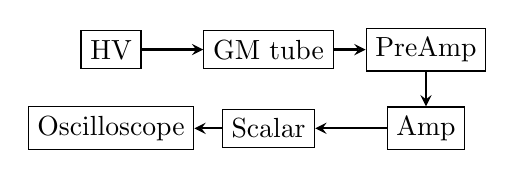
\begin{tikzpicture}[node distance=.65cm]
			%http://www.texample.net/tikz/examples/feature/arrows/
			\usetikzlibrary{shapes.geometric, arrows} 
			\tikzstyle{startstop} = [rectangle, rounded corners, minimum width=.2cm, minimum height=.2cm,text centered, draw=black]
			\tikzstyle{rect} = [rectangle, minimum width=.2cm, minimum height=.2cm, text centered, draw=black]%, fill=orange!30]
			\tikzstyle{parallelogram} = [diamond, minimum width=.2cm, minimum height=.2cm, text centered,draw=black]
			\tikzstyle{arrow} = [thick,->,>=stealth]

			\node (HV) at (0,2) [rect] {HV};
			\node (GM) at (2,2) [rect] {GM tube};
			\node (pre) at (4,2) [rect] {PreAmp};
			\node (amp) at (4,1) [rect] {Amp};
			\node (count) at (2,1) [rect] {Scalar};
			\node (osc) at (0,1) [rect] {Oscilloscope};

			\draw [arrow] (HV) -- (GM);
			\draw [arrow] (GM) -- (pre);
			\draw [arrow] (pre) -- (amp);
			\draw [arrow] (amp) -- (count);
			\draw [arrow] (count) -- (osc);

			%\draw [dashed, arrow] (Cname) -- (Iname);

		\end{tikzpicture}
		\caption{\small{The electronics used in this apparatus are labeled in this schematic. \label{fig:aparatuslatex}}}
		\end{center}
	\end{figure}


Background detections were established by collecting data over the full angular range, with no crystal.  To account for angular dependent background, detections recorded with no crystal were subtracted from data collected using NaCl and LiF crystals.  
%To account for uneven background counts, the full angular range used during data collection was scanned with no source.  
Background from scattered X-rays were minimized by placing small pieces of lead around the apparatus.  While collecting data, the Amp introduced significant noise, causing its removal from the final experimental apparatus.

\section{Data}
\iffalse
	%NEWER DATA RESULTS
	\begin{figure}
	\begin{center}
		%\input{NaCl_part1}
		\centerline{% GNUPLOT: LaTeX picture with Postscript
\begingroup
  \makeatletter
  \providecommand\color[2][]{%
    \GenericError{(gnuplot) \space\space\space\@spaces}{%
      Package color not loaded in conjunction with
      terminal option `colourtext'%
    }{See the gnuplot documentation for explanation.%
    }{Either use 'blacktext' in gnuplot or load the package
      color.sty in LaTeX.}%
    \renewcommand\color[2][]{}%
  }%
  \providecommand\includegraphics[2][]{%
    \GenericError{(gnuplot) \space\space\space\@spaces}{%
      Package graphicx or graphics not loaded%
    }{See the gnuplot documentation for explanation.%
    }{The gnuplot epslatex terminal needs graphicx.sty or graphics.sty.}%
    \renewcommand\includegraphics[2][]{}%
  }%
  \providecommand\rotatebox[2]{#2}%
  \@ifundefined{ifGPcolor}{%
    \newif\ifGPcolor
    \GPcolortrue
  }{}%
  \@ifundefined{ifGPblacktext}{%
    \newif\ifGPblacktext
    \GPblacktextfalse
  }{}%
  % define a \g@addto@macro without @ in the name:
  \let\gplgaddtomacro\g@addto@macro
  % define empty templates for all commands taking text:
  \gdef\gplbacktext{}%
  \gdef\gplfronttext{}%
  \makeatother
  \ifGPblacktext
    % no textcolor at all
    \def\colorrgb#1{}%
    \def\colorgray#1{}%
  \else
    % gray or color?
    \ifGPcolor
      \def\colorrgb#1{\color[rgb]{#1}}%
      \def\colorgray#1{\color[gray]{#1}}%
      \expandafter\def\csname LTw\endcsname{\color{white}}%
      \expandafter\def\csname LTb\endcsname{\color{black}}%
      \expandafter\def\csname LTa\endcsname{\color{black}}%
      \expandafter\def\csname LT0\endcsname{\color[rgb]{1,0,0}}%
      \expandafter\def\csname LT1\endcsname{\color[rgb]{0,1,0}}%
      \expandafter\def\csname LT2\endcsname{\color[rgb]{0,0,1}}%
      \expandafter\def\csname LT3\endcsname{\color[rgb]{1,0,1}}%
      \expandafter\def\csname LT4\endcsname{\color[rgb]{0,1,1}}%
      \expandafter\def\csname LT5\endcsname{\color[rgb]{1,1,0}}%
      \expandafter\def\csname LT6\endcsname{\color[rgb]{0,0,0}}%
      \expandafter\def\csname LT7\endcsname{\color[rgb]{1,0.3,0}}%
      \expandafter\def\csname LT8\endcsname{\color[rgb]{0.5,0.5,0.5}}%
    \else
      % gray
      \def\colorrgb#1{\color{black}}%
      \def\colorgray#1{\color[gray]{#1}}%
      \expandafter\def\csname LTw\endcsname{\color{white}}%
      \expandafter\def\csname LTb\endcsname{\color{black}}%
      \expandafter\def\csname LTa\endcsname{\color{black}}%
      \expandafter\def\csname LT0\endcsname{\color{black}}%
      \expandafter\def\csname LT1\endcsname{\color{black}}%
      \expandafter\def\csname LT2\endcsname{\color{black}}%
      \expandafter\def\csname LT3\endcsname{\color{black}}%
      \expandafter\def\csname LT4\endcsname{\color{black}}%
      \expandafter\def\csname LT5\endcsname{\color{black}}%
      \expandafter\def\csname LT6\endcsname{\color{black}}%
      \expandafter\def\csname LT7\endcsname{\color{black}}%
      \expandafter\def\csname LT8\endcsname{\color{black}}%
    \fi
  \fi
    \setlength{\unitlength}{0.0500bp}%
    \ifx\gptboxheight\undefined%
      \newlength{\gptboxheight}%
      \newlength{\gptboxwidth}%
      \newsavebox{\gptboxtext}%
    \fi%
    \setlength{\fboxrule}{0.5pt}%
    \setlength{\fboxsep}{1pt}%
\begin{picture}(5040.00,3772.00)%
    \gplgaddtomacro\gplbacktext{%
      \csname LTb\endcsname%
      \put(682,704){\makebox(0,0)[r]{\strut{}$0$}}%
      \put(682,971){\makebox(0,0)[r]{\strut{}$10$}}%
      \put(682,1239){\makebox(0,0)[r]{\strut{}$20$}}%
      \put(682,1506){\makebox(0,0)[r]{\strut{}$30$}}%
      \put(682,1774){\makebox(0,0)[r]{\strut{}$40$}}%
      \put(682,2041){\makebox(0,0)[r]{\strut{}$50$}}%
      \put(682,2309){\makebox(0,0)[r]{\strut{}$60$}}%
      \put(682,2576){\makebox(0,0)[r]{\strut{}$70$}}%
      \put(682,2844){\makebox(0,0)[r]{\strut{}$80$}}%
      \put(682,3111){\makebox(0,0)[r]{\strut{}$90$}}%
      \put(1069,484){\makebox(0,0){\strut{}$56$}}%
      \put(1580,484){\makebox(0,0){\strut{}$58$}}%
      \put(2090,484){\makebox(0,0){\strut{}$60$}}%
      \put(2601,484){\makebox(0,0){\strut{}$62$}}%
      \put(3111,484){\makebox(0,0){\strut{}$64$}}%
      \put(3622,484){\makebox(0,0){\strut{}$66$}}%
      \put(4132,484){\makebox(0,0){\strut{}$68$}}%
      \put(4643,484){\makebox(0,0){\strut{}$70$}}%
    }%
    \gplgaddtomacro\gplfronttext{%
      \csname LTb\endcsname%
      \put(176,1907){\rotatebox{-270}{\makebox(0,0){\strut{}Intensity [counts]}}}%
      \put(2728,154){\makebox(0,0){\strut{}2$\theta$ [deg]}}%
      \put(2728,3441){\makebox(0,0){\strut{}NaCl: n=2}}%
      \csname LTb\endcsname%
      \put(3656,2938){\makebox(0,0)[r]{\strut{}Ni Filter}}%
      \csname LTb\endcsname%
      \put(3656,2718){\makebox(0,0)[r]{\strut{}No Filter}}%
    }%
    \gplbacktext
    \put(0,0){\includegraphics{NaCl_part2}}%
    \gplfronttext
  \end{picture}%
\endgroup
}
		\caption{\small{Sodium-Chloride with various filters, at n=2. \label{fig:NaCln2}}}
	\end{center}
	\end{figure}

	\begin{table}[H]
		\begin{center}
			\begin{tabular}{ | c | c | c | c | c | }\hline
			Crystal & Filter & Experimental & Theoretical & $\sigma$ \\ \hline
			NaCl & none & $57.745\pm0.201$ & & \\ \hline
			NaCl & none & $64.887\pm0.105$ & & \\ \hline%NaCl & none & $64.887\pm0.1046$ & & \\ \hline
			NaCl & Ni & $64.827\pm14.630$ & & \\ \hline
			LiF & Ni & & & \\ \hline
			\end{tabular}
		\end{center}
	\caption{ \small{Lattice constant values for NaCl and LiF, with n=2.  \label{tab:ne2}}}
	\end{table}
\fi

%In order to calculate the lattice constants of NaCl and LiF, the weighted average of angles on the $n=1$ and $n=2$ lines were taken~\cite{she}.  Lack of detector sensitivity made it impossible to distinguish between the $K_{\alpha_{1}}$ and $K_{\alpha_{2}}$ peaks, in our data.  For comparison to theoretical literature, a weighted average of the angles these peaks occur at was also taken~\cite{daichi}.
In order to calculate the lattice constants of NaCl and LiF, the weighted average of angles at which these peaks occur was taken, on the $n=1$ and $n=2$ lines~\cite{she}.  Lack of detector sensitivity made it impossible to distinguish between the $K_{\alpha_{1}}$ and $K_{\alpha_{2}}$ peaks, in our data.  For comparison to theoretical literature, a weighted average of the angles these peaks occur at was also taken~\cite{daichi}.

Nickel has a K-absorption edge at $148.8~pm$, causing it to absorb radiation from Cu~$K_{\beta}$ much more strongly than it absorbs Cu~$K_{\alpha}$ radiation~\cite{she}.  By taking data with and without a Ni filter, the $K_{\alpha}$ peaks isolated.
%For this reason, a Ni filter was used to isolate the $K_{alpha}$ peaks.  

%\begin{center}
%	$\mu = \frac{\sum x_{i} / \sigma_{i}^{2}}{\sum 1 / \sigma_{i}^2}$
%\end{center}
\iffalse
	\begin{table}[H]
		\begin{center}
			\begin{tabular}{ | c | c | c | c | }\hline
			Crystal & Filter & Peak & Experimental \\ \hline
			NaCl & none & $K_{\beta}$ & $26.94\pm0.002$ \\ \hline
			NaCl & none & $K_{\alpha}$ & $30.15\pm27.04$ \\ \hline
			NaCl & Ni & $K_{\alpha}$ & $30.16\pm0.07$ \\ \hline
			LiF & None & $K_{\beta}$ & $39.51\pm0.04$ \\ \hline
			LiF & None &  $K_{\alpha}$ & $44.12\pm0.35$ \\ \hline
			LiF & Ni & $K_{\alpha}$ & $44.09\pm0.10$ \\ \hline
			\end{tabular}
		\end{center}
	\caption{ \small{$K_{\alpha}$ and $K_{\beta}$ peak values for NaCl and LiF, with n=1.  \label{tab:ne1}}}
	\end{table}

	\begin{table}[H]
		\begin{center}
			\begin{tabular}{ | c | c | c | c | }\hline
			Crystal & Filter & Peak & Experimental \\ \hline
			NaCl & none & $K_{\beta}$ & $60.96\pm5.32$ \\ \hline
			NaCl & none & $K_{\alpha}$ & $65.00\pm0.12$ \\ \hline
			NaCl & Ni & $K_{\alpha}$ & $64.99\pm6.94$ \\ \hline
			LiF & none & $K_{\beta}$ & $86.56\pm5.54$ \\ \hline
			LiF & Ni & $K_{\alpha}$ & $30.69\pm42.08$ \\ \hline
			\end{tabular}
		\end{center}
	\caption{ \small{$K_{\alpha}$ and $K_{\beta}$ peak values for NaCl and LiF, with n=2.  \label{tab:ne2}}}
	\end{table}
\fi

%%% TABLE n=1
\begin{table}[H]
	\begin{center}
	%\resizebox{\columnwidth}{!}{%
	\begin{tabular}{ |c|c|c| } 
	 \hline
	 \multicolumn{3}{|c|}{NaCl} \\ 
	 \hline
				Peak & Filter & Measured Angle \\ \hline
				$K_{\beta}$ & none & $26.94\pm0.002$ \\ \hline
				$K_{\alpha}$ & none & $30.15\pm27.04$ \\ \hline
				~~~$K_{\alpha}$~~~&~~~Ni~~~&~~~$30.16\pm0.07$~~~\\ \hline
	\hline \hline
	 \multicolumn{3}{|c|}{LiF} \\
	 \hline
		Peak & Filter & Measured Angle \\ \hline
		$K_{\beta}$ & none & $39.51\pm0.04$ \\ \hline
		$K_{\alpha}$ & none & $44.12\pm0.35$ \\ \hline
		~~~$K_{\alpha}$~~~&~~~Ni~~~&~~~$44.09\pm0.10$~~~\\ \hline
	\end{tabular}
	\caption{ \small{$K_{\alpha}$ and $K_{\beta}$ peak values for NaCl and LiF, with n=1. \label{tab:ne1}}}
	\end{center}
	%\label{tab:ne1}
	%}
\end{table}

%%% TABLE n=2
\begin{table}[H]
	\begin{center}
	%\resizebox{\columnwidth}{!}{%
	\begin{tabular}{ |c|c|c| } 
	 \hline
	 \multicolumn{3}{|c|}{NaCl} \\ 
	 \hline
			Peak & Filter & Measured Angle \\ \hline
			$K_{\beta}$ & none & $60.96\pm5.32$ \\ \hline
			$K_{\alpha}$ & none & $65.00\pm0.12$ \\ \hline
			~~~$K_{\alpha}$~~~&~~~Ni~~~&~~~$64.99\pm6.94$~~~\\ \hline
	\hline \hline
	 \multicolumn{3}{|c|}{LiF} \\
	 \hline
			Peak & Filter & Measured Angle \\ \hline
			~~~$K_{\beta}$~~~&~~~none~~~&~~~$86.56\pm5.54$~~~\\ \hline
			%~~~$K_{\alpha}$~~~&~~~Ni~~~&~~~$30.69\pm42.08$~~~\\ \hline
	\end{tabular}
	\caption{ \small{$K_{\alpha}$ and $K_{\beta}$ peak values for NaCl and LiF, with n=2. \label{tab:ne2}}}
	\end{center}
	%}
\end{table}

%%INTENSITY
\begin{figure}[H]
	\begin{center}
		\centerline{\includegraphics[width=3in]{figures/intensity}}
		\caption{\small{Intensity as a function of wavelength. \label{fig:intensity}}}
	\end{center}
\end{figure}

Figure~\ref{fig:intensity}~\cite{daichi} shows that $K_{\beta}$ peaks occur at lower wavelengths with lower intensities than $K_{\alpha}$ peaks.  For Copper the $K_{\alpha_{1}}$, $K_{\alpha_{2}}$, and $K_{\beta}$ X-ray lines occur at $154.0~pm$, $154.4~pm$, and $139.2~pm$, respectively~\cite{she}.


\subsection{NaCl}

%% RAW DATA
	%\begin{figure}[H]
	%	\begin{center}
	%		\centerline{\includegraphics[width=3in]{figures/NaCl.png}}
	%		\caption{\small{NaCl with no and Ni filter. \label{fig:NaCl}}}
	%	\end{center}
	%\end{figure}	
Tables~\ref{tab:ne1}~and~\ref{tab:ne2} list the $2\theta$ values corresponding to observed $K_{\alpha}$ and $K_{\beta}$ peaks, for NaCl.  Figures~\ref{fig:NaCln1}~and~\ref{fig:NaCln2} show collected data with Gaussian fits, for NaCl at $n=1$ and $n=2$, respectively.
% DETERMINED WITHOUT USING NI FILTER K\alpha VALUES IN WEIGHT MEAN
%The lattice constant of NaCl was experimentally determined to be $(599.89\pm35.32)~pm$ with a deviation of $1.02\sigma$, from the accepted value of $564.02~pm$.

\begin{figure}[H]
	\begin{center}
		%\input{NaCl_part1}
		\centerline{\input{testeps}}
		\caption{\small{NaCl with various filters, at n=1. \label{fig:NaCln1}}}
	\end{center}
\end{figure}

\begin{figure}[H]
	\begin{center}
		\centerline{\input{NaCl_older}}
		\caption{\small{NaCl with various filters, at n=2. \label{fig:NaCln2}}}
	\end{center}
\end{figure}





\vfill\eject


\subsection{LiF}

%Figure~\ref{fig:LiFn2} shows the data taken using LiF at $n=2$.  
$K_{\beta}$ peaks occur at lower angles than $K_{\alpha}$ peaks.  Due to the detector's limited angle range, no $K_{\alpha}$ was observed for LiF with $n=2$, shown by Figure~\ref{fig:LiFn2}.  The $K_{\alpha}$ peak is expected to occur at $2\theta=100^{\circ}$, but the apparatus could only achieve a maximum of $2\theta=95^{\circ}$.

%% RAW DATA
	%\begin{figure}[H]
	%	\begin{center}
	%		\centerline{\includegraphics[width=3in]{figures/LiF.png}}
	%		\caption{\small{Lithium-Floride with no and Ni filter. \label{fig:LiF}}}
	%	\end{center}
	%\end{figure}	

\begin{figure}[H]
	\begin{center}
		%\input{NaCl_part1}
		\centerline{% GNUPLOT: LaTeX picture with Postscript
\begingroup
  \makeatletter
  \providecommand\color[2][]{%
    \GenericError{(gnuplot) \space\space\space\@spaces}{%
      Package color not loaded in conjunction with
      terminal option `colourtext'%
    }{See the gnuplot documentation for explanation.%
    }{Either use 'blacktext' in gnuplot or load the package
      color.sty in LaTeX.}%
    \renewcommand\color[2][]{}%
  }%
  \providecommand\includegraphics[2][]{%
    \GenericError{(gnuplot) \space\space\space\@spaces}{%
      Package graphicx or graphics not loaded%
    }{See the gnuplot documentation for explanation.%
    }{The gnuplot epslatex terminal needs graphicx.sty or graphics.sty.}%
    \renewcommand\includegraphics[2][]{}%
  }%
  \providecommand\rotatebox[2]{#2}%
  \@ifundefined{ifGPcolor}{%
    \newif\ifGPcolor
    \GPcolortrue
  }{}%
  \@ifundefined{ifGPblacktext}{%
    \newif\ifGPblacktext
    \GPblacktextfalse
  }{}%
  % define a \g@addto@macro without @ in the name:
  \let\gplgaddtomacro\g@addto@macro
  % define empty templates for all commands taking text:
  \gdef\gplbacktext{}%
  \gdef\gplfronttext{}%
  \makeatother
  \ifGPblacktext
    % no textcolor at all
    \def\colorrgb#1{}%
    \def\colorgray#1{}%
  \else
    % gray or color?
    \ifGPcolor
      \def\colorrgb#1{\color[rgb]{#1}}%
      \def\colorgray#1{\color[gray]{#1}}%
      \expandafter\def\csname LTw\endcsname{\color{white}}%
      \expandafter\def\csname LTb\endcsname{\color{black}}%
      \expandafter\def\csname LTa\endcsname{\color{black}}%
      \expandafter\def\csname LT0\endcsname{\color[rgb]{1,0,0}}%
      \expandafter\def\csname LT1\endcsname{\color[rgb]{0,1,0}}%
      \expandafter\def\csname LT2\endcsname{\color[rgb]{0,0,1}}%
      \expandafter\def\csname LT3\endcsname{\color[rgb]{1,0,1}}%
      \expandafter\def\csname LT4\endcsname{\color[rgb]{0,1,1}}%
      \expandafter\def\csname LT5\endcsname{\color[rgb]{1,1,0}}%
      \expandafter\def\csname LT6\endcsname{\color[rgb]{0,0,0}}%
      \expandafter\def\csname LT7\endcsname{\color[rgb]{1,0.3,0}}%
      \expandafter\def\csname LT8\endcsname{\color[rgb]{0.5,0.5,0.5}}%
    \else
      % gray
      \def\colorrgb#1{\color{black}}%
      \def\colorgray#1{\color[gray]{#1}}%
      \expandafter\def\csname LTw\endcsname{\color{white}}%
      \expandafter\def\csname LTb\endcsname{\color{black}}%
      \expandafter\def\csname LTa\endcsname{\color{black}}%
      \expandafter\def\csname LT0\endcsname{\color{black}}%
      \expandafter\def\csname LT1\endcsname{\color{black}}%
      \expandafter\def\csname LT2\endcsname{\color{black}}%
      \expandafter\def\csname LT3\endcsname{\color{black}}%
      \expandafter\def\csname LT4\endcsname{\color{black}}%
      \expandafter\def\csname LT5\endcsname{\color{black}}%
      \expandafter\def\csname LT6\endcsname{\color{black}}%
      \expandafter\def\csname LT7\endcsname{\color{black}}%
      \expandafter\def\csname LT8\endcsname{\color{black}}%
    \fi
  \fi
    \setlength{\unitlength}{0.0500bp}%
    \ifx\gptboxheight\undefined%
      \newlength{\gptboxheight}%
      \newlength{\gptboxwidth}%
      \newsavebox{\gptboxtext}%
    \fi%
    \setlength{\fboxrule}{0.5pt}%
    \setlength{\fboxsep}{1pt}%
\begin{picture}(5040.00,3772.00)%
    \gplgaddtomacro\gplbacktext{%
      \csname LTb\endcsname%
      \put(946,704){\makebox(0,0)[r]{\strut{}$-200$}}%
      \put(946,945){\makebox(0,0)[r]{\strut{}$0$}}%
      \put(946,1185){\makebox(0,0)[r]{\strut{}$200$}}%
      \put(946,1426){\makebox(0,0)[r]{\strut{}$400$}}%
      \put(946,1667){\makebox(0,0)[r]{\strut{}$600$}}%
      \put(946,1908){\makebox(0,0)[r]{\strut{}$800$}}%
      \put(946,2148){\makebox(0,0)[r]{\strut{}$1000$}}%
      \put(946,2389){\makebox(0,0)[r]{\strut{}$1200$}}%
      \put(946,2630){\makebox(0,0)[r]{\strut{}$1400$}}%
      \put(946,2870){\makebox(0,0)[r]{\strut{}$1600$}}%
      \put(946,3111){\makebox(0,0)[r]{\strut{}$1800$}}%
      \put(1078,484){\makebox(0,0){\strut{}$30$}}%
      \put(1969,484){\makebox(0,0){\strut{}$35$}}%
      \put(2861,484){\makebox(0,0){\strut{}$40$}}%
      \put(3752,484){\makebox(0,0){\strut{}$45$}}%
      \put(4643,484){\makebox(0,0){\strut{}$50$}}%
    }%
    \gplgaddtomacro\gplfronttext{%
      \csname LTb\endcsname%
      \put(176,1907){\rotatebox{-270}{\makebox(0,0){\strut{}Intensity [counts]}}}%
      \put(2860,154){\makebox(0,0){\strut{}2$\theta$ [deg]}}%
      \put(2860,3441){\makebox(0,0){\strut{}LiF: n=1}}%
      \csname LTb\endcsname%
      \put(2398,2938){\makebox(0,0)[r]{\strut{}No Filter}}%
      \csname LTb\endcsname%
      \put(2398,2718){\makebox(0,0)[r]{\strut{}Ni Filter}}%
    }%
    \gplbacktext
    \put(0,0){\includegraphics{LiF_n1}}%
    \gplfronttext
  \end{picture}%
\endgroup
}
		\caption{\small{LiF with various filters, at n=1. \label{fig:LiFn1}}}
	\end{center}
\end{figure}

\begin{figure}[H]
	\begin{center}
		%\input{NaCl_part1}
		\centerline{\input{LiF_n2}}
		\caption{\small{LiF with various filters, at n=2. \label{fig:LiFn2}}}
	\end{center}
\end{figure}


%The $2\theta$ values corresponding to observed $K_{\alpha}$ and $K_{\beta}$ peaks for LiF at $n=1$ and $n=2$, shown in Figures~\ref{fig:LiFn1}~and~\ref{fig:LiFn2}, are listed in Tables~\ref{tab:ne1}~and~\ref{tab:ne2}, respectively.

Tables~\ref{tab:ne1}~and~\ref{tab:ne2} list the $2\theta$ values corresponding to observed $K_{\alpha}$ and $K_{\beta}$ peaks, for LiF.  Figures~\ref{fig:LiFn1}~and~\ref{fig:LiFn2} show collected data with Gaussian fits, for LiF at $n=1$ and $n=2$, respectively.




\section{Results and Analysis}

The lattice constant of NaCl was experimentally determined to be $(521.17\pm67.11)~pm$. This deviates by $0.64\sigma$, from the accepted value of $564.02~pm$~\cite{anacl}.  The lattice constant of LiF was experimentally determined to be $(428.44\pm177.10)~pm$ with a deviation of $0.15\sigma$, from the accepted value of $402.6~pm$~\cite{alif}.  Minor variation between experimental and theoretical values are likely due to crystal orientation.  If not seated perfectly, the diffraction patterns will occur at angles offset from theoretical values.




%\vfill\eject % clear column
%\clearpage % clear column (sometimes) or page

\setlength{\parindent}{0cm}
%\bibliographystyle{plain}
\bibliographystyle{apsrev}
%\bibliography{biblio} % uses bib items in external 'biblio.bib' file
%\bibliographystyle{aipauth4-1}

%\bibliographystyle{revtex4}




\begin{thebibliography}{99}
~\\ % so there is a space between affiliations and bib items

\bibitem{crystal} Cambridge Physics - X-ray Diffraction. (n.d.). Retrieved March 20, 2016, from \url{http://www.outreach.phy.cam.ac.uk/camphy/xraydiffraction/xraydiffraction_index.htm} \\

\bibitem{daichi} Cockcroft, J. K. (2006). Generation of X-rays. Retrieved March 20, 2016, from \url{http://pd.chem.ucl.ac.uk/pdnn/inst1/xrays.htm} \\

\bibitem{she} \url{http://www.phys.hawaii.edu/~shige/phys481L/XRay.txt} \\

\bibitem{alif} Lithium Fluoride (LiF). (2013). Retrieved March 19, 2016, from \url{http://www.mateck.com/} \\

\bibitem{book} Melissinos, A. \& Napolitano, J. (2003). \textit{Experiments in modern physics, 2nd Ed}. San Diego: Academic Press. \\

\bibitem{anacl} Toreki, R. (2015, March 30). Structure World. Retrieved March 19, 2016, from \url{http://www.ilpi.com/inorganic/structures/nacl/} \\

\end{thebibliography}



\end{document}

